
\begin{frame}{ElGamal Permutations}

For $p$ prime, $\Z_p^* = \{1, \ldots, p-1\}$ is a cyclic group of order $p-1$ under multiplication. For $g$ a generator, the ElGamal map $x \to g^x$ from $\Z_p^*$ to $\Z_p^*$ is a permutation
\vspace{1cm}

\begin{itemize}
\item The ElGamal function is the basis of the ElGamal Signature Scheme
  \item The ElGamal function used in the Welch construction of Costas Arrays
  \end{itemize}

  
\end{frame}




\begin{frame}{Research challenge}

In 2016 Joachim von zur Gathen posed this research challenge:

\begin{itemize}
    \item Let $a,b,c \overset{?}{\gets} \mathbb{Z}_p^*$.
    \item DDH assumption: ($g^a, g^b, g^{ab}$) $\sim$ ($g^a, g^b, g^c$)
\end{itemize}

\pause
\vspace{10pt}
\begin{center}
    {\Large
        How random is the ElGamal map?
        
        Is $ (x, g^x) \sim  (x, x')$  when $x,x' \overset{?}{\gets} \mathbb{Z}_p^*$?
    }
\end{center}

\pause
\vspace{10pt}
    We proceed showing some evidence from (Niehues et al., 2020)

\end{frame}




\begin{frame}{Cycles in ElGamal Permutations}
Example: The generators of $\Z_5^*$ are  $2$ and $3$.

    \begin{columns}
        \begin{column}{0.45\textwidth}
        \centering
    	    \begin{tabular}{c|c}
    	        $x$ & $g^{x} $ \\ \hline \hline
    	        $1$ & $2^{1} = 2$ \\
    	        $2$ & $2^{2} = 4$ \\
    	        $3$ & $2^{3} = 3$ \\
              $4$ & $2^{4} = 1$  \\
                \multicolumn{2}{c}{} \\
              \multicolumn{2}{c}{$\gamma = (1,2,4)(3)$}
    	    \end{tabular}
        \end{column}
        \begin{column}{0.45\textwidth}
    	    \centering
    	    \begin{tabular}{c|c}
    	        $x$ & $g^{x} $ \\ \hline \hline
    	        $1$ & $3^{1} = 3$ \\
    	        $2$ & $3^{2} = 4$ \\
    	        $3$ & $3^{3} = 2$ \\
    	        $4$ & $3^{4} = 1$  \\
                \multicolumn{2}{c}{} \\
              \multicolumn{2}{c}{$\gamma  = (1,2,3,4)$}
    	    \end{tabular}
        \end{column}
  \end{columns}
  \vspace{1cm}
  
  \pause
  \begin{itemize}
      \item Distinct $g$ produce distinct permutations;
      \item Distinct $g$ affect the cyclic structures.
  \end{itemize}
  
\end{frame}

\begin{frame}{$p = 1009$}
\begin{tabular}{cc}
\begin{tabular}{c}
  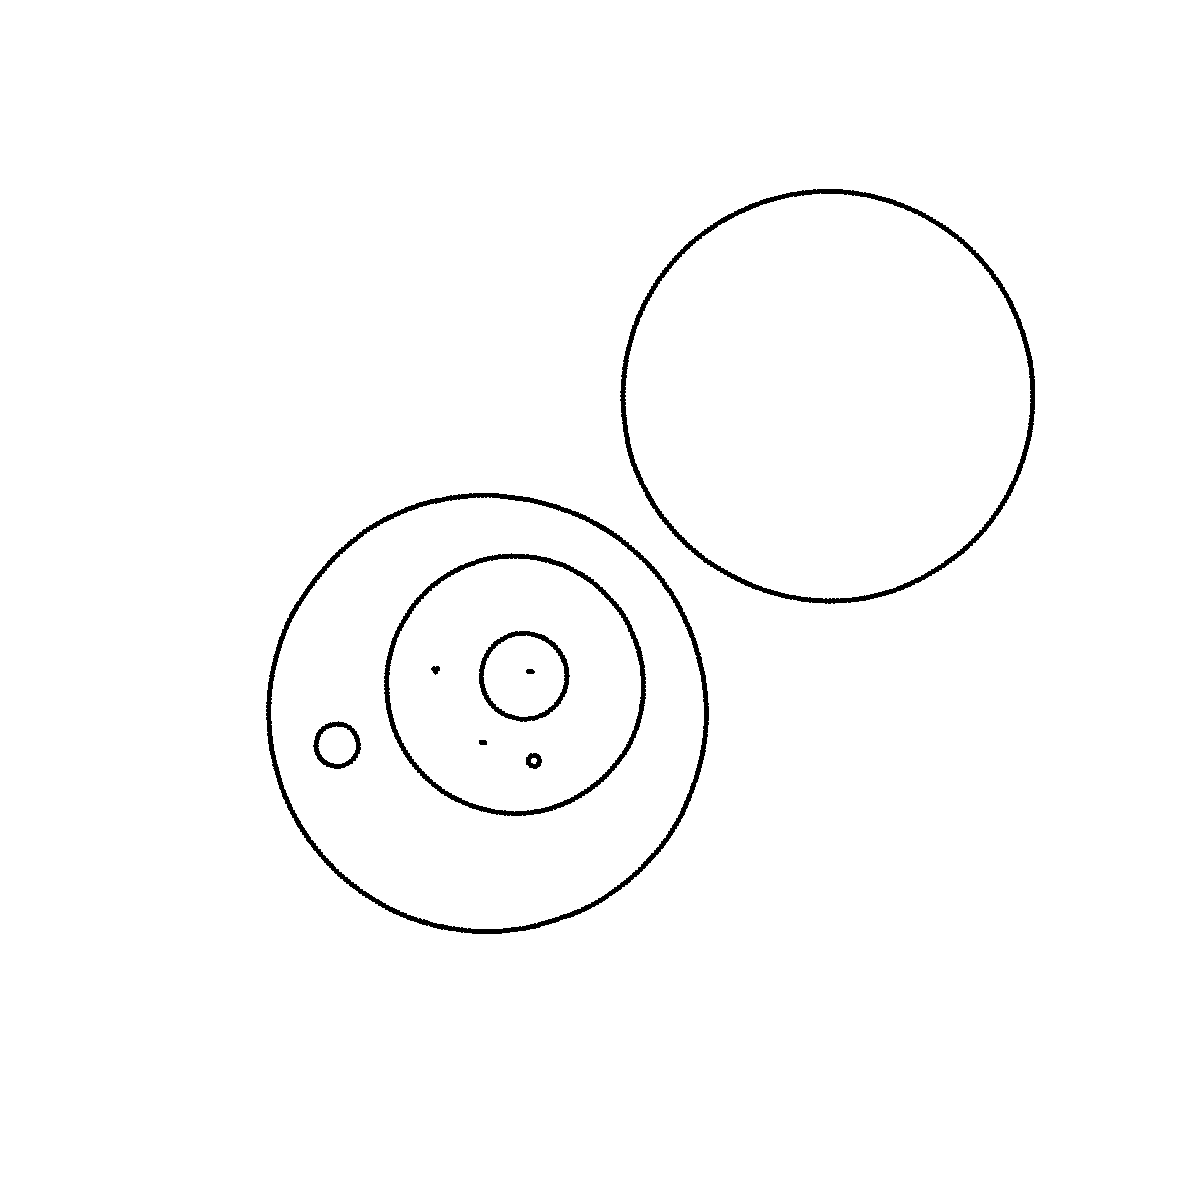
\includegraphics[height=0.4\textwidth]{figures/graph_0011_1009.pdf}\\[-1cm]
  $g=11$
  \end{tabular}
  &
\begin{tabular}{c}
\raisebox{0.5cm}{        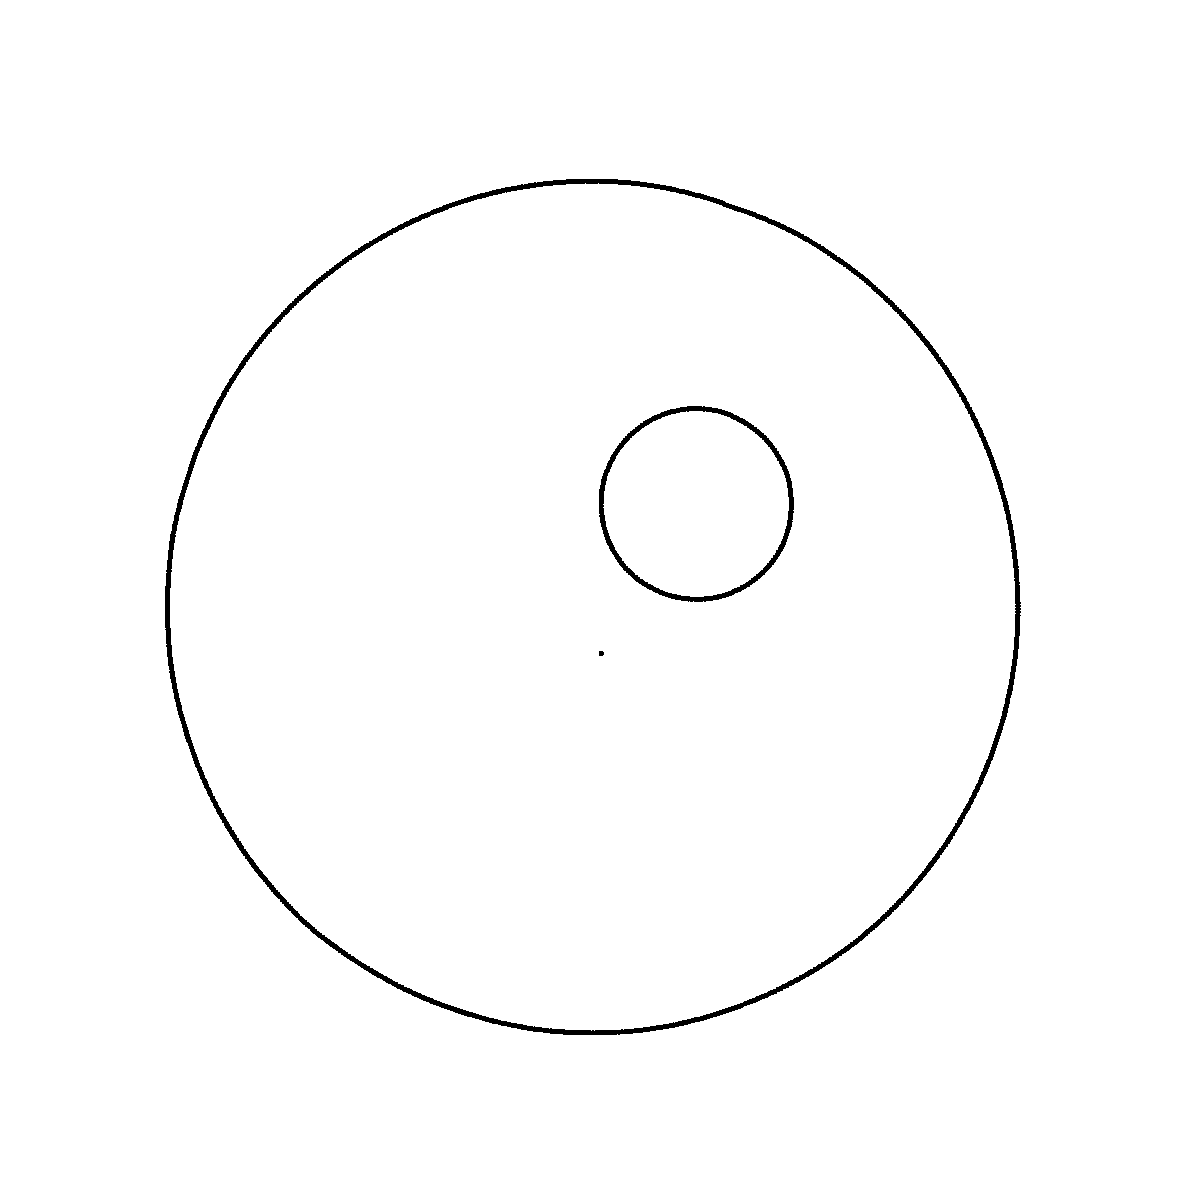
\includegraphics[width=0.4\textwidth]{figures/graph_0017_1009.pdf}}\\[-1.3cm]
  $g=17$
  \end{tabular}
  \\[0cm]
\begin{tabular}{c}
        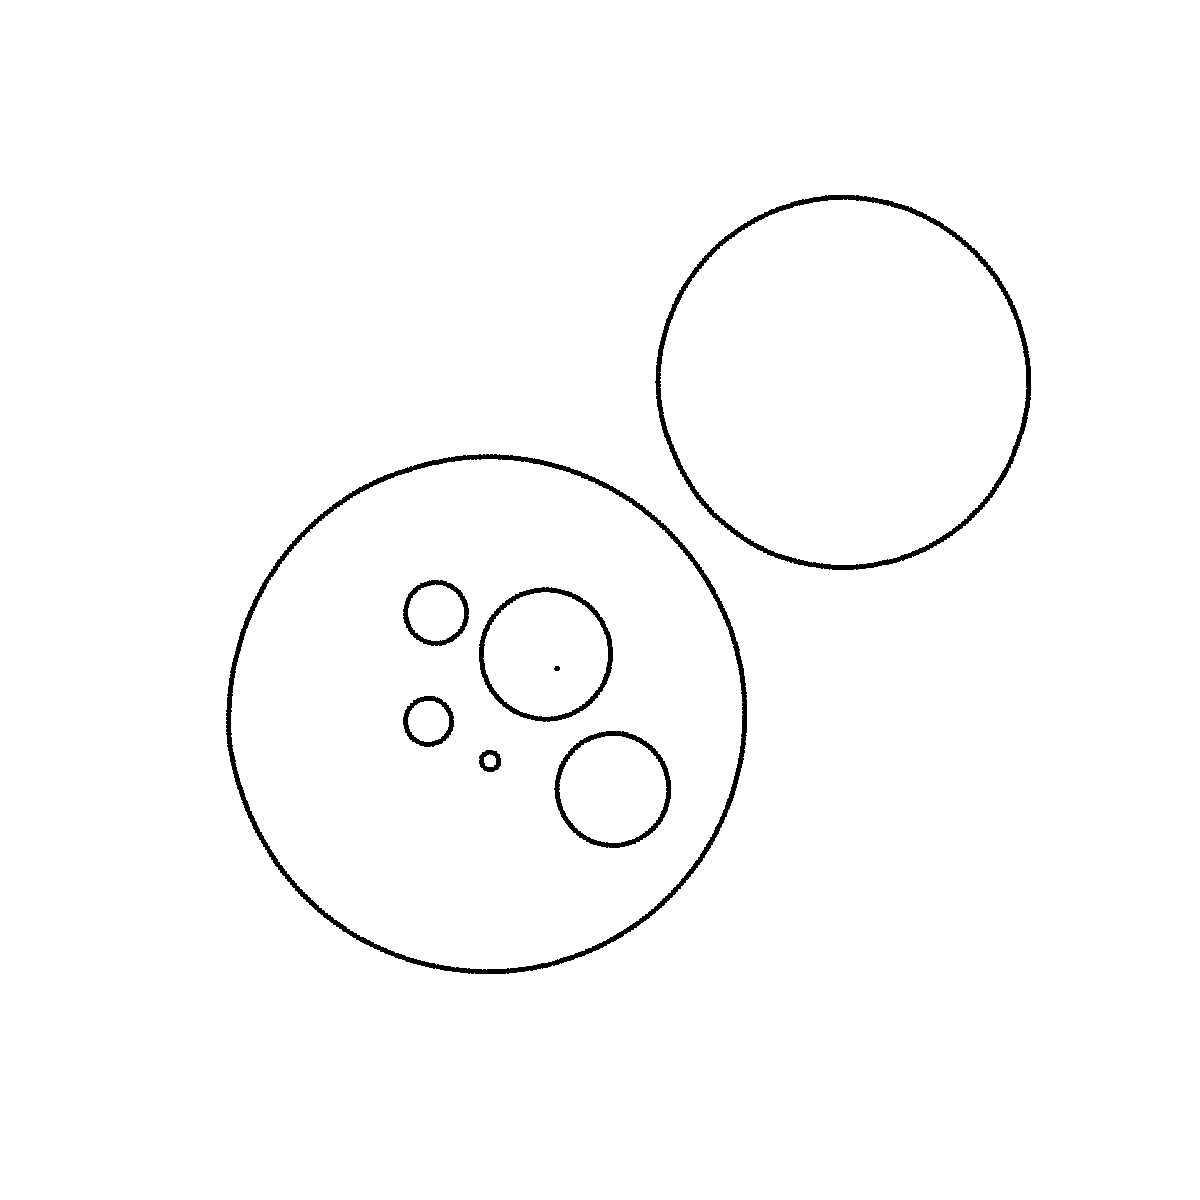
\includegraphics[width=0.4\textwidth]{figures/graph_0022_1009.pdf}\\[-1cm]
  $g=22$
  \end{tabular}
  &
\begin{tabular}{c}
        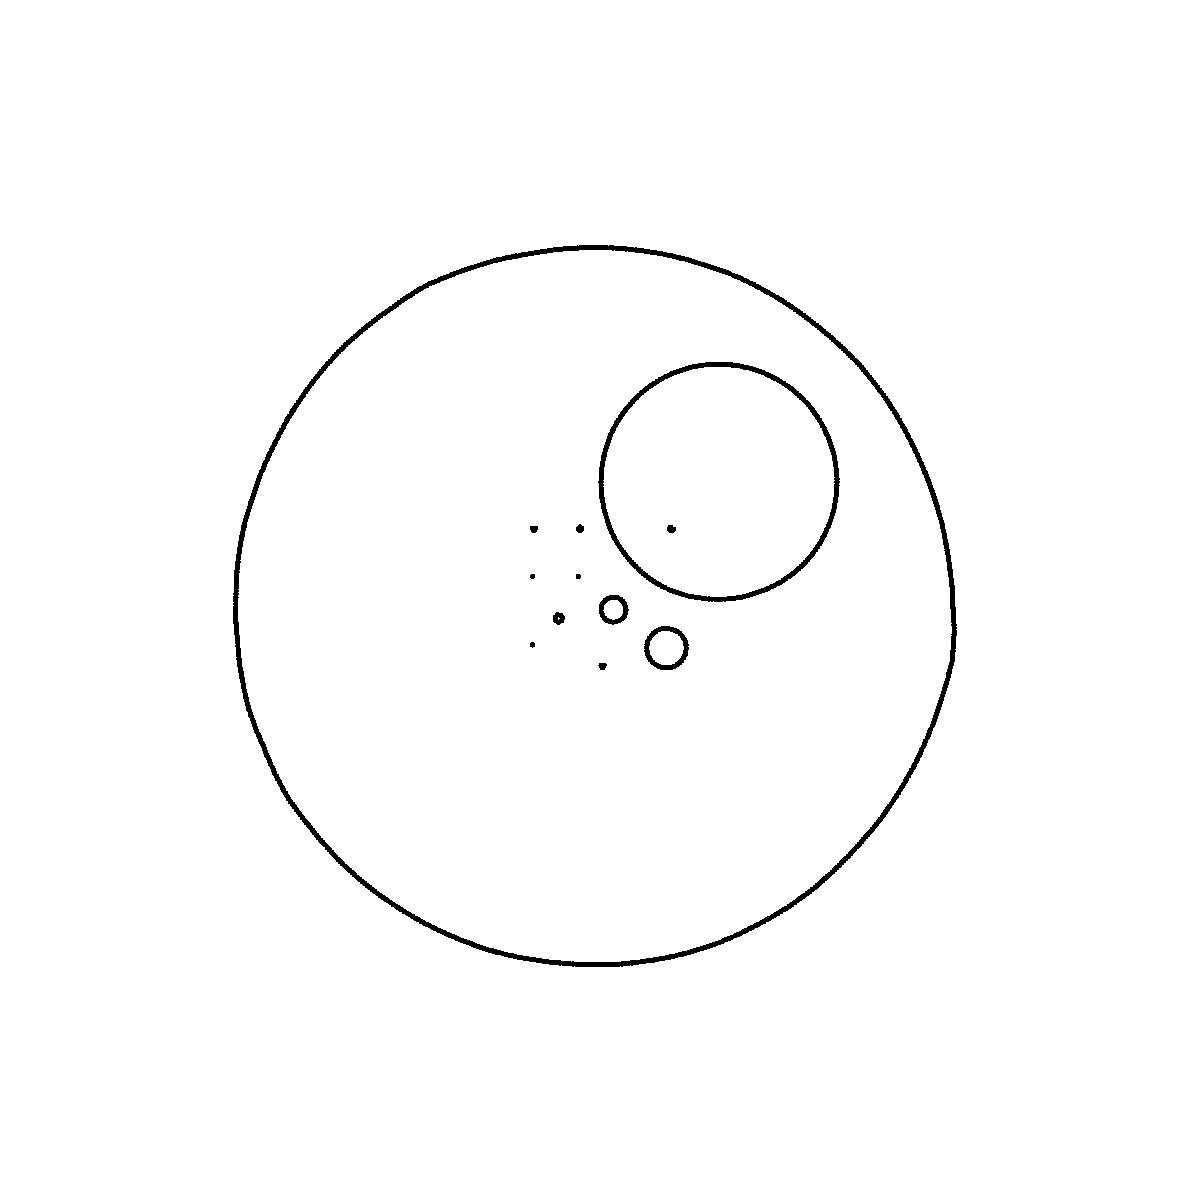
\includegraphics[width=0.4\textwidth]{figures/graph_0026_1009.pdf}\\[-1cm]
  $g=26$
  \end{tabular}
\end{tabular}
\end{frame}

\begin{frame}{Number of cycles}
        \centering
        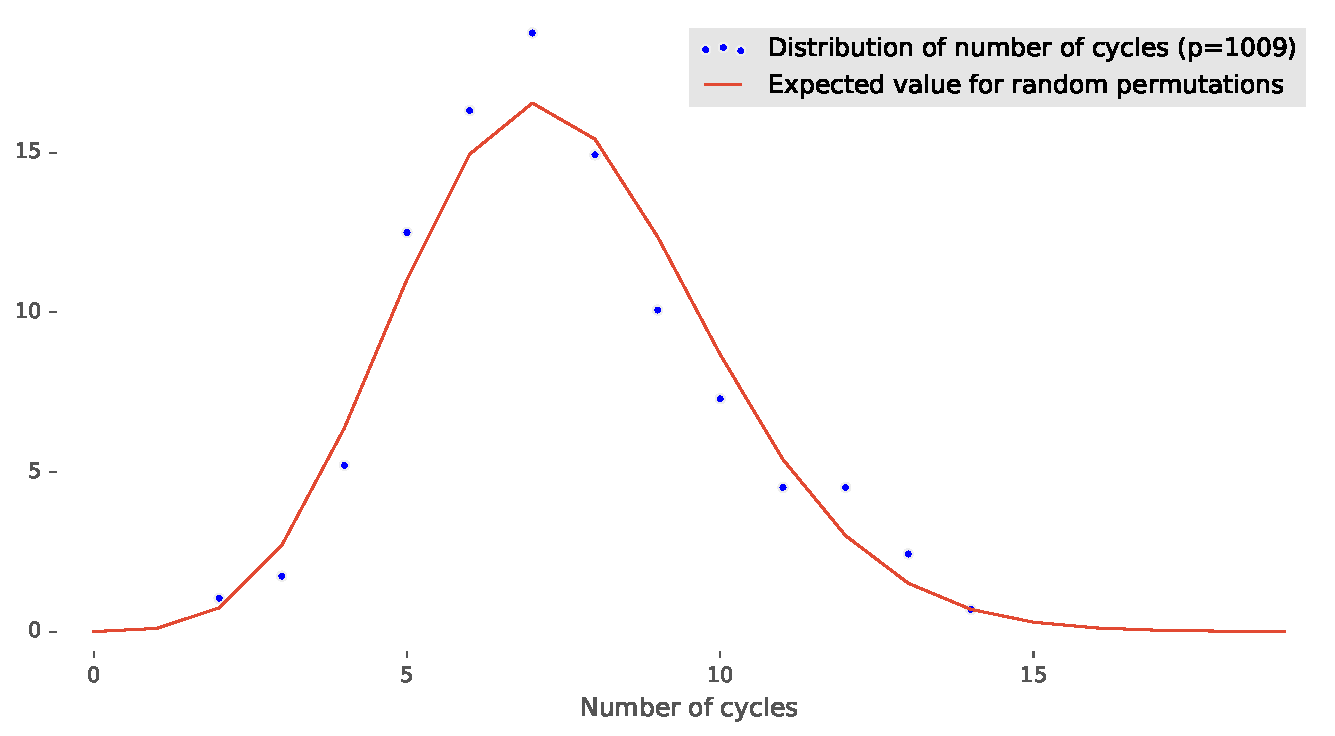
\includegraphics[width=\textwidth]{figures/distribution_of_number_of_cycles_p_1009}\\
 {Distribution of number of cycles for all 288 generators of $\mathbb{F}_{1009}$}
\end{frame}

\begin{frame}{Number of $k$-cycles}
        \centering
        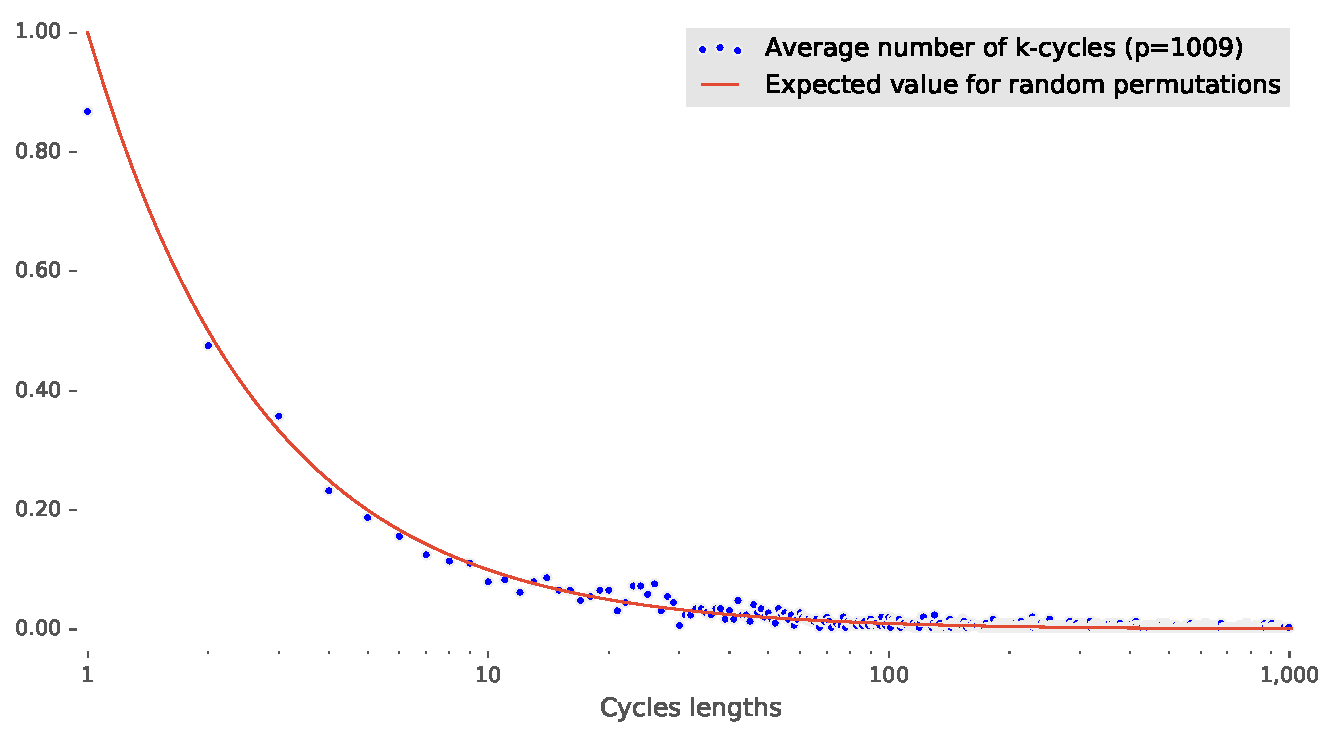
\includegraphics[width=\textwidth]{figures/average_number_of_k_cycles_p_1009}\\
{Average number of $k$-cycles in $\mathbb{F}_{1009}$}
\end{frame}

\begin{frame}{Number of fixed points ($k=1$)}
        \centering
        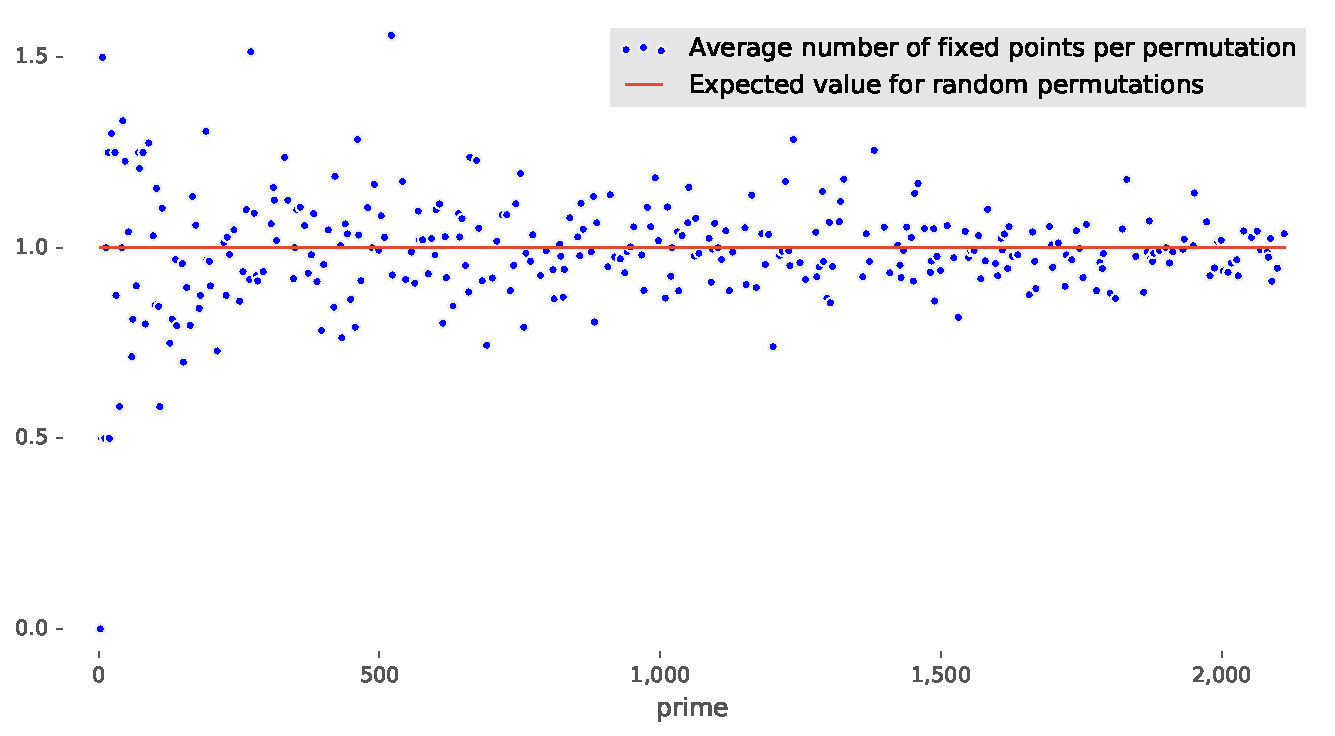
\includegraphics[width=\textwidth]{figures/average_number_of_fixed_points_per_permutation}\\
{Average number of fixed points in the generators of $\mathbb{F}_p$}
\end{frame}


\begin{frame}{Results with Sidon Sets}
  Let $S = \{(x,g^x): x \in \mathbb{Z}_p^*\}$ be the graph of the ElGamal permutation. Because $S$ is a Sidon Set,

  \begin{theorem}[Niehues et al., 2020]
    Let
    \[
      B = [h_1,\ldots, h_2] \times [k_1,\ldots k_2] \subset \mathbb{Z}_p^* \times \mathbb{Z}_p.
    \]
    Then
    \[
      \left | \cardinality{S \cup B} - \frac{\cardinality{B}}{p} \right | \leq 50 p^{1/2} \log^2 p
\]
    \end{theorem}
\end{frame}

\begin{frame}{Other randomness properties}

  \begin{itemize}
  \item Drakakis et al. prove the ElGamal function is {\em Almost Perfect Nonlinear}
    \item Closer to PN than most APN functions in differential uniformity
    \item More linear than most Costas functions on a log-ratio test
      \item Less linear than random functions with a phase modulation test 
    \end{itemize}
  
  \end{frame}



\begin{frame}{Sequences from permutations}
    \begin{center}
        {\Large
            How random sequences?
        }
    \end{center}
    
    \pause
    For any  permutation $\pi$ in $\mathbb{Z}_p^*$, make a sequence
    \[
        \pi_v = (\pi_1 \rem v, \ldots, \pi_{p-1}\rem v).
    \]
    
    \pause

    Example:  $p=5$ and $g=2$
    \begin{align*}            \gamma &= ( (2^0) \rem 5) \rem 2, \ldots, (2^3) \rem 5) \rem 2)\\
      &= (1, 2, 4, 3) \\
        \gamma_2 &= (1, 0, 0, 1) \in \mathbb{Z}_2^4
    \end{align*}
\end{frame}


\begin{frame}{Randomness properties of ElGamal Sequences?}
    
    \begin{center}
        How closely do ElGamal sequences compare to sequences from random permutations?
    \end{center}
    
    \begin{itemize}
        \item Balance
        \item Period length
        \item Distribution of fixed $t$-\emph{tuples} $z\in\mathbb{Z}_v^t$:
        $$\lambda(z) = \cardinality{\{i \in [0,p-1]: \gamma_v(i+_{n} \iota) = z(\iota),\; 0 \leq \iota < t\}}$$
        \item  Distribution of \emph{runs} of $b\in\mathbb{Z}_v$ and of length $t$:
        \begin{align*}
            \rho(b,t) = & \cardinality{ \{i \in [0,p-1]: }\\
                        &\gamma_v(i-_{n} 1),\gamma_v(i+_n t) \neq b = \gamma_v(i+_n\iota),\; 0 \leq \iota < t\}
        \end{align*}
        \item $\rho(t) = v \rho(t+1)$
        % $\rho(b,t) = \cardinality{ \{i \in [0,p-1]: \sigma(i-_{n} 1),\sigma(i+_n t) \neq b = \sigma(i+_n\iota),\; 0 \leq \iota < t\}}$
    \end{itemize}
  
  \end{frame}

  \begin{frame}{Other uses of Modulo operator in sequences}

    \begin{itemize}
      \item The Legendre sequence
      \[
(\log_g(i) \rem 2, \log_g(i+1) \rem 2, \ldots )      
        \]
      \item  Colbourn constructed covering arrays from the circulant matrix
      \[
(\log_g(i) \rem v, \log_g(i+1) \rem v, \ldots )      
        \]
      \item Tzanakis et al. formed covering array from circulant matrices of
        \[
(\log_g( tr(g^i)) \rem v, \log_g( tr(g^{i+1})) \rem v, \ldots )      
        \]
      \end{itemize}
    
    \end{frame}


  

%%% Local Variables:
%%% TeX-master: "../main.tex"
%%% End: